\documentclass[a4paper,12pt]{article}
\usepackage[left=2.5cm, right=2.5cm, top=3cm, bottom=3cm]{geometry}
\usepackage[spanish]{babel}
\usepackage{graphicx}
\usepackage[utf8]{inputenc}

\begin{document}
\title{Presentación del Proyecto}
\author{Barabaro Yoel Martinez Gonalez C113}

\maketitle
\begin{figure}[h]
	\center
	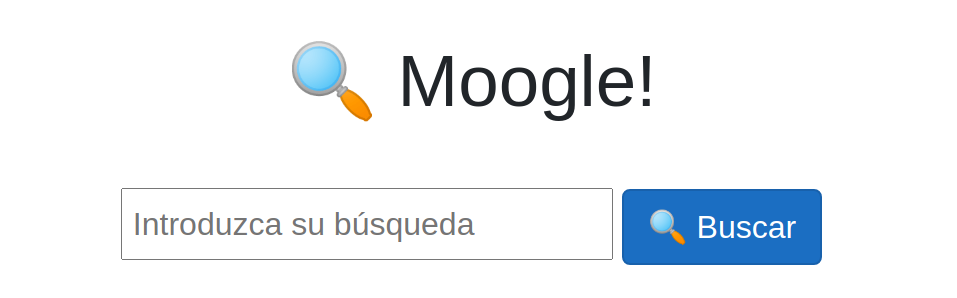
\includegraphics[width=8cm]{moogle.png}
	\caption{Moogle!}
	\label{fig:logo}
\end{figure}
\section{Como funciona el buscador?}



\begin{flushleft}
El buscador funciona cargando archivos txt, leyendolos y metiendolos en un array q luego cada palabra de estas terminara en un diccionario como una llave. A todo esto se le quitan los caracteres extraños y los caracteres vacíos. Al implementar una búsqueda se le hace lo mismo al contenido de la busqueda pero se tiene en cuenta la relevancia de cada palabra. Las palabras en un array de un archivo se pasan por un metodo que calculara el TF que va a tener como valor la cantidad de veces que aparece la palabra en un archivo. El idf nos dara la aparicion de la palabra a nivel de carpeta mediante un diccionario llamdo AllTFs que tendra como llave el string con el nombre del archivo y como valor otro diccionario q tendrá las palabras de los archivos y cuántas veces aparecen. Si la búsqueda es vacia tendrá una notificación de ello y se le dirá que hacer. Si no se encuentra lo que buscó simplemente el buscador devolverá una búsqueda vacía


\end{flushleft}
\end{document}
